\documentclass[aspectratio=169]{beamer}
\PassOptionsToPackage{english}{babel}
\usepackage{standardslides}

\usepackage{svg}

\usepackage{tikz}
\usepackage{pifont}
\usepackage{listings}
\usepackage{colortbl}
\newlength{\listingframemargin}
\setlength{\listingframemargin}{1em}
\newlength{\listingmargin}
\setlength{\listingmargin}{0.08\textwidth}

\definecolor{codeDarkGray}{gray}{0.2}
\definecolor{codeGray}{gray}{0.4}
\definecolor{codeLightGray}{rgb}{0.94,0.94,0.91}
\definecolor{codeBorder}{rgb}{0.34,0.24,0.21}
\definecolor{MidnightBlue}{rgb}{0.1, 0.1, 0.8}

\lstdefinestyle{standard}{%
  belowcaptionskip=0.5\baselineskip,
  breaklines=true,
  frameround=tttt,
  % frame=false,
  xleftmargin=0em,
  xrightmargin=0em,
  showstringspaces=false,
  showtabs=false,
  % tab=\smash{\rule[-.2\baselineskip]{.4pt}{\baselineskip}\kern.5em},
  basicstyle= \fontfamily{pcr}\selectfont\tiny\bfseries,
  keywordstyle= \bfseries\color{MidnightBlue}, %\color{codeDarkGray},
  commentstyle= \itshape\color{codeGray},
  identifierstyle=\color{codeDarkGray},
  stringstyle=\color{BurntOrange}, %\color{codeDarkGray},
  numberstyle=\tiny\ttfamily,
  % numbers=left,
  numbersep = 1em,
  % stepnumber = 1,
  % captionpos=t,
  tabsize=2,
  % backgroundcolor=\color{codebLightGray},
  rulecolor=\color{codeBorder},
  framexleftmargin=\listingframemargin,
  framexrightmargin=\listingframemargin
}

\newcommand{\inputCodeBlock}[1]{%
  % \begin{mybox}
    \begin{center}
      % \begin{minipage}[c]{0.7\textwidth}
        \lstinputlisting[%
          style = standard,
          language = c++,
          morekeywords={constexpr,noexcept,decltype,size_t,uint32_t,uint64_t,__m256i,__m256,__m256d,__m128i,__m128,__m128d}
        ]{#1}
      % \end{minipage}
    \end{center}
  % \end{mybox}
}

\def\UrlBigBreaks{\do\/\do-\do:}

\setbeamertemplate{footline}[frame number]
\setbeamertemplate{navigation symbols}{}

\title{%
  Probabilistic Circuits: \\ Marginal Maximum a Posteriori Queries%
}
% \subtitle{Master's Thesis Defense and Presentation}
\author{Markus Pawellek}

\bibliography{references}

\DeclareMathOperator*{\argmax}{arg\ max}
\DeclareMathOperator{\val}{val}
\DeclareMathOperator{\nodein}{in}

\begin{document}

\selectlanguage{english}

\frame[plain]{\titlepage}
\begin{frame}[plain]{Outline}
  \footnotesize
  \hfill\parbox[t][7cm][l]{0.9\textwidth}{\tableofcontents}
\end{frame}
\setcounter{framenumber}{0}

\section{Introduction}
  \begin{frame}{Introduction}
    \begin{itemize}
      \item Marginal maximum a posteriori (MMAP) combine marginal (MAR) and maximum a posteriori (MAP) inference
      \item We need sufficient conditions for tractability
      \item We use MAR and MAP algorithm
      \item Notations varies a little bit: no boldface letters
    \end{itemize}
  \end{frame}

\section{Background}
  \begin{frame}{Background}
    \begin{align*}
      X &\ldots \text{finite set of random variables} \\
      p\, &\ldots \text{joint probability distribution over $X$} \\
      \mathscr{C}\, &\ldots \text{PC over $X$ with $\mathscr{C}=(\mathscr{G},ϑ)$} \\
      Q &\ldots \text{set of query variables with $Q\subset X$}
    \end{align*}
  \end{frame}

  \begin{frame}{Background: MMAP Queries}
    \begin{itemize}
      \item query variables $Q$, evidence variables $E$, marginal variables $Z$ form partition of $X$
      \item $e\in E$, intevals $\mathscr{I}\subset\val(Z)$
    \end{itemize}
    \begin{mybox}
      \[
        \argmax_{q\in\val(Q)} \ p\roundBrackets{Q=q \ | \ E=e,Z\in\mathscr{I}}
      \]
      \[
        \argmax_{q\in\val(Q)} \integral{\mathscr{I}}{}{p(q,e,z)}{Z}
      \]
    \end{mybox}
  \end{frame}

  \begin{frame}{Background: MMAP Connection}
    \begin{mybox}
      \[
        \argmax_{q\in\val(Q)} \integral{\mathscr{I}}{}{p(q,e,z)}{Z}
      \]
    \end{mybox}
    \begin{itemize}
      \item $\mathbf{case}\ Q=\emptyset :\quad $ MAR Query
      \[
        \integral{\mathscr{I}}{}{p(e,z)}{Z}
      \]
      \item $\mathbf{case}\ Z=\emptyset :\quad $ MAP Query
      \[
        \argmax_{q\in\val(Q)}\ p(q,e)
      \]
    \end{itemize}
  \end{frame}

  \begin{frame}{Background: Review}
    \[
      \begin{aligned}[t]
        &\text{$\mathscr{C}$ is tractable for MAR queries} \\
        &\iff \text{$\mathscr{G}$ is decomposable and smooth}
      \end{aligned}
    \]
    \[
      \begin{aligned}[t]
        &\text{$\mathscr{C}$ is tractable for MAP queries} \\
        &\iff \text{$\mathscr{G}$ is consistent and deterministic}
      \end{aligned}
    \]
    \[
      \text{$\mathscr{G}$ is decomposable} \implies \text{$\mathscr{G}$ is consistent}
    \]
    \begin{mybox}
      \begin{align*}
        &\text{$\mathscr{C}$ is tractable for both MAR and MAP queries} \\
        &\iff \text{$\mathscr{G}$ is decomposable, smooth, and deterministic }
      \end{align*}
    \end{mybox}
  \end{frame}

\section{Marginal Determinism}
  \begin{frame}{Marginal Determinism}
    \begin{mybox}
      A sum node is marginal deterministic with respect to $Q$ if for all partial states $q\in Q$ at most one of its inputs is non-zero.
    \end{mybox}
    \begin{mybox}
      A circuit structure $\mathscr{G}$ is marginal deterministic with respect to $Q$ if for all sum units $n\in\mathscr{G}$ with $φ(n)\cap Q\neq\emptyset$, $n$ is marginal deterministic with respect to $Q$.
    \end{mybox}
    \begin{itemize}
      \item Simple generalization of determinism
      \item Structural property about the support of input units
      \item Defined with respect to $Q$
    \end{itemize}
  \end{frame}

  \begin{frame}{Marginal Determinism: Example}
    \center
    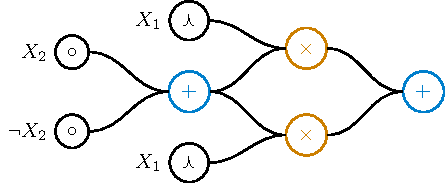
\includegraphics[width=0.9\textwidth]{figures/example.pdf}
  \end{frame}
  \begin{frame}{Marginal Determinism: Example}
    \center
    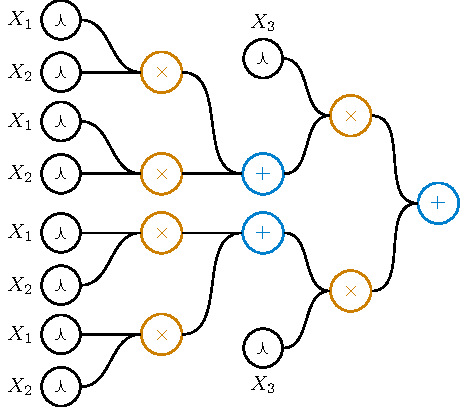
\includegraphics[height=0.8\textheight]{figures/big-example.pdf}
  \end{frame}

\section{Tractable Computation}
  \begin{frame}{Tractable Computation: General}
    \begin{itemize}
      \item<+-> Adjust feed-forward algorithms for MAR and MAP queries
      \item<+-> At the end, backward pass is needed for modes
      \item<+-> Assume, input units provide correct output \\[1em]
      \begin{center}
        
\includegraphics{figures/input-unit.pdf}
      \end{center}
      \item<+-> Product units are handled identically in MAR and MAP \\[1em]
      \begin{minipage}[c]{0.4\textwidth}
        \begin{mybox}
          \[
            r_n \longleftarrow \prod_{c\in\nodein(n)} r_c
          \]
        \end{mybox}
      \end{minipage}
      \hfill
      \begin{minipage}[c]{0.45\textwidth}
        \centering
        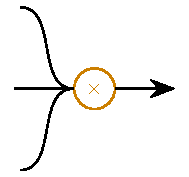
\includegraphics{figures/product-unit.pdf}
      \end{minipage}
    \end{itemize}
  \end{frame}

  \begin{frame}{Tractable Computation: Sum Units}
    \begin{minipage}[c]{0.49\textwidth}
      \begin{mybox}
        \begin{align*}
          \mathbf{if}\quad &φ(n) \cap Q \neq \emptyset \quad \mathbf{then} \\
          & r_n \longleftarrow \max_{c\in\nodein(n)} ϑ_{nc}r_c \\
          \mathbf{else} \\
          & r_n \longleftarrow \sum_{c\in\nodein(n)} ϑ_{nc}r_c
        \end{align*}
      \end{mybox}
    \end{minipage}
    \hfill
    \begin{minipage}[c]{0.49\textwidth}
      \center
      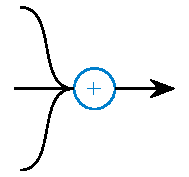
\includegraphics[scale=1.2]{figures/sum-unit.pdf}
    \end{minipage}
  \end{frame}

\section{Sufficient Conditions}
  \begin{frame}{Sufficient Conditions}
    \begin{mybox}
      \textbf{Theorem:}
      Let $\mathscr{G}$ be smooth, decomposable, and $Q$-marginal deterministic.
      Then for any parameterization $ϑ$ the above algorithm
      tractably computes MMAP queries of $\mathscr{C}$ over $Q$.
    \end{mybox}
    \begin{itemize}
      \item Proof by induction
      \item Input units are correct by assumption
    \end{itemize}
    \[
      \mathscr{Q}(e,\mathscr{I}) = \max_{q\in\val(Q)} \integral{\mathscr{I}}{}{\mathscr{C}(Z,q,e)}{Z}
    \]
  \end{frame}

  \begin{frame}{Sufficient Conditions: Product Units}
    \begin{itemize}
      \item<+-> Apply decomposability and partition $Z$, $Q$, and $E$
    \end{itemize}
    \begin{align*}
      \uncover<+->{\mathscr{Q}(e,\mathscr{I}) &= \max_{q_1,\ldots,q_k\in\val(Q)} \integral{\mathscr{I}}{}{\prod_{i=1}^k\mathscr{C}_i(Z_i,q_i,e_i)}{Z} }\\
      \uncover<+->{&= \max_{q_1,\ldots,q_k\in\val(Q)} \prod_{i=1}^k \integral{\mathscr{I}}{}{\mathscr{C}_i(Z_i,q_i,e_i)}{Z_i} }\\
      \uncover<+->{&= \prod_{i=1}^k \max_{q_i\in\val(Q)} \integral{\mathscr{I}_i}{}{\mathscr{C}_i(Z_i,q_i,e_i)}{Z_i} }\\
      \uncover<+->{&= \prod_{i=1}^k \mathscr{C}_i(e_i,\mathscr{I}_i) }
    \end{align*}
  \end{frame}

  \begin{frame}{Sufficient Conditions: Sum Units}
    \begin{itemize}
      \item<+-> Sum units with no query variable in their scope reduce to MAR queries which has alread been proven
      \item<+-> So $φ(n)\cap Q \neq \emptyset$
    \end{itemize}
    \begin{align*}
      \uncover<+->{\mathscr{Q}(e,\mathscr{I}) &= \max_{q\in\val(Q)} \integral{\mathscr{I}}{}{\sum_{i\in\nodein(n)} ϑ_i\mathscr{C}_i(Z,q,e)}{Z} }\\
      \uncover<+->{&= \max_{q\in\val(Q)} \sum_{i\in\nodein(n)} \integral{\mathscr{I}}{}{ϑ_i\mathscr{C}_i(Z,q,e)}{Z} }\\
      \uncover<+->{&= \max_{q\in\val(Q)} \max_{i\in\nodein(n)} \integral{\mathscr{I}}{}{ϑ_i\mathscr{C}_i(Z,q,e)}{Z} }\\
      \uncover<+->{&= \max_{i\in\nodein(n)} ϑ_i \max_{q\in\val(Q)} \integral{\mathscr{I}}{}{\mathscr{C}_i(Z,q,e)}{Z} }\\
      \uncover<+->{&= \max_{i\in\nodein(n)} ϑ_i \mathscr{Q}_i(e,\mathscr{I})}
    \end{align*}
  \end{frame}

\section{Conclusions}
  \begin{frame}{Conclusions}
    \begin{itemize}
      \item<+-> MMAP queries are typically be NP-hard
      \item<+-> Complexity depends on set of query variables
      \item<+-> marginal determinism together with smoothness and decomposability seems to be sufficient for tractable computations
      \item<+-> sum units have to compute maxima when support contains query variables
    \end{itemize}
  \end{frame}

  \begin{frame}{Conclusions: Outlook}
    \uncover<5->{%
      \begin{beamercolorbox}[sep=8pt,center,shadow=true,rounded=true]{title}
        \usebeamerfont{title}%
        Thank you for Your Attention!%
        \par%
      \end{beamercolorbox}%
    }%
    \vspace{1em}
    \onslide<+->
    \begin{minipage}[c]{0.49\textwidth}
      \center
      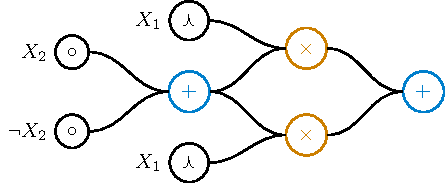
\includegraphics[width=\textwidth]{figures/example.pdf}
    \end{minipage}
    \begin{minipage}[c]{0.49\textwidth}
      \begin{itemize}
        \item<+-> Marginal determinism for all sets of query variables
        \item<+-> Sum-maximizer circuits (no general algorithm)
        \item<+-> Tractable computation of information-theoretic measures
      \end{itemize}
    \end{minipage}
  \end{frame}

\setcounter{backupcounter}{\value{framenumber}}

\begin{frame}[plain]
  \frametitle{References}
  % \tiny
  % \AtNextBibliography{\tiny}
  % \begin{multicols}{2}
    \nocite{*}
    \printbibliography
  % \end{multicols}
\end{frame}

\setcounter{framenumber}{\value{backupcounter}}

\end{document}
